% Chapter 12

\chapter{Comparación Modelo de la ANN} % Write in your own chapter title
\label{Chapter12}
\lhead{Capítulo 12. \emph{Comparación ANN}} % Write in your own chapter

%En este capítulo se analizarán comparativamente los niveles de detección entre un modelo de ANN usando las herramientas de Matlab (nntool) y el modelo en hardware propuesto en este documento en el Capítulo \ref{Chapter6}, Figura \ref{fig:MLP}. El objetivo es demostrar que el modelo propuesto es válido y puede ser implementado a nivel de hardware directamente. Para esto se eligió mostrar la detección del modelo de la red en punto fijo usando el entrenamiento de Matlab con especificaciones iguales a las del modelo Hardware propuesto. Por otra parte, se usó el entrenamiento directamente sobre el modelo hardware usando C/C++.

Es importante mencionar que el rendimiento de una ANN depende directamente de la calidad del entrenamiento y del conjunto de datos elegido. Por lo tanto, en este capítulo se analizarán comparativamente los niveles de detección entre un modelo de ANN usando las herramientas de Matlab (nntool) frente al modelo en hardware propuesto en este documento en el Capítulo \ref{Chapter10}, Figura \ref{fig:networkDesign}. El objetivo es demostrar que el modelo propuesto es válido y puede ser implementado a nivel de hardware directamente. Para esto se eligió mostrar la detección del modelo de la red en punto fijo usando el entrenamiento de Matlab.

\begin{figure}[!ht]
	\centering
		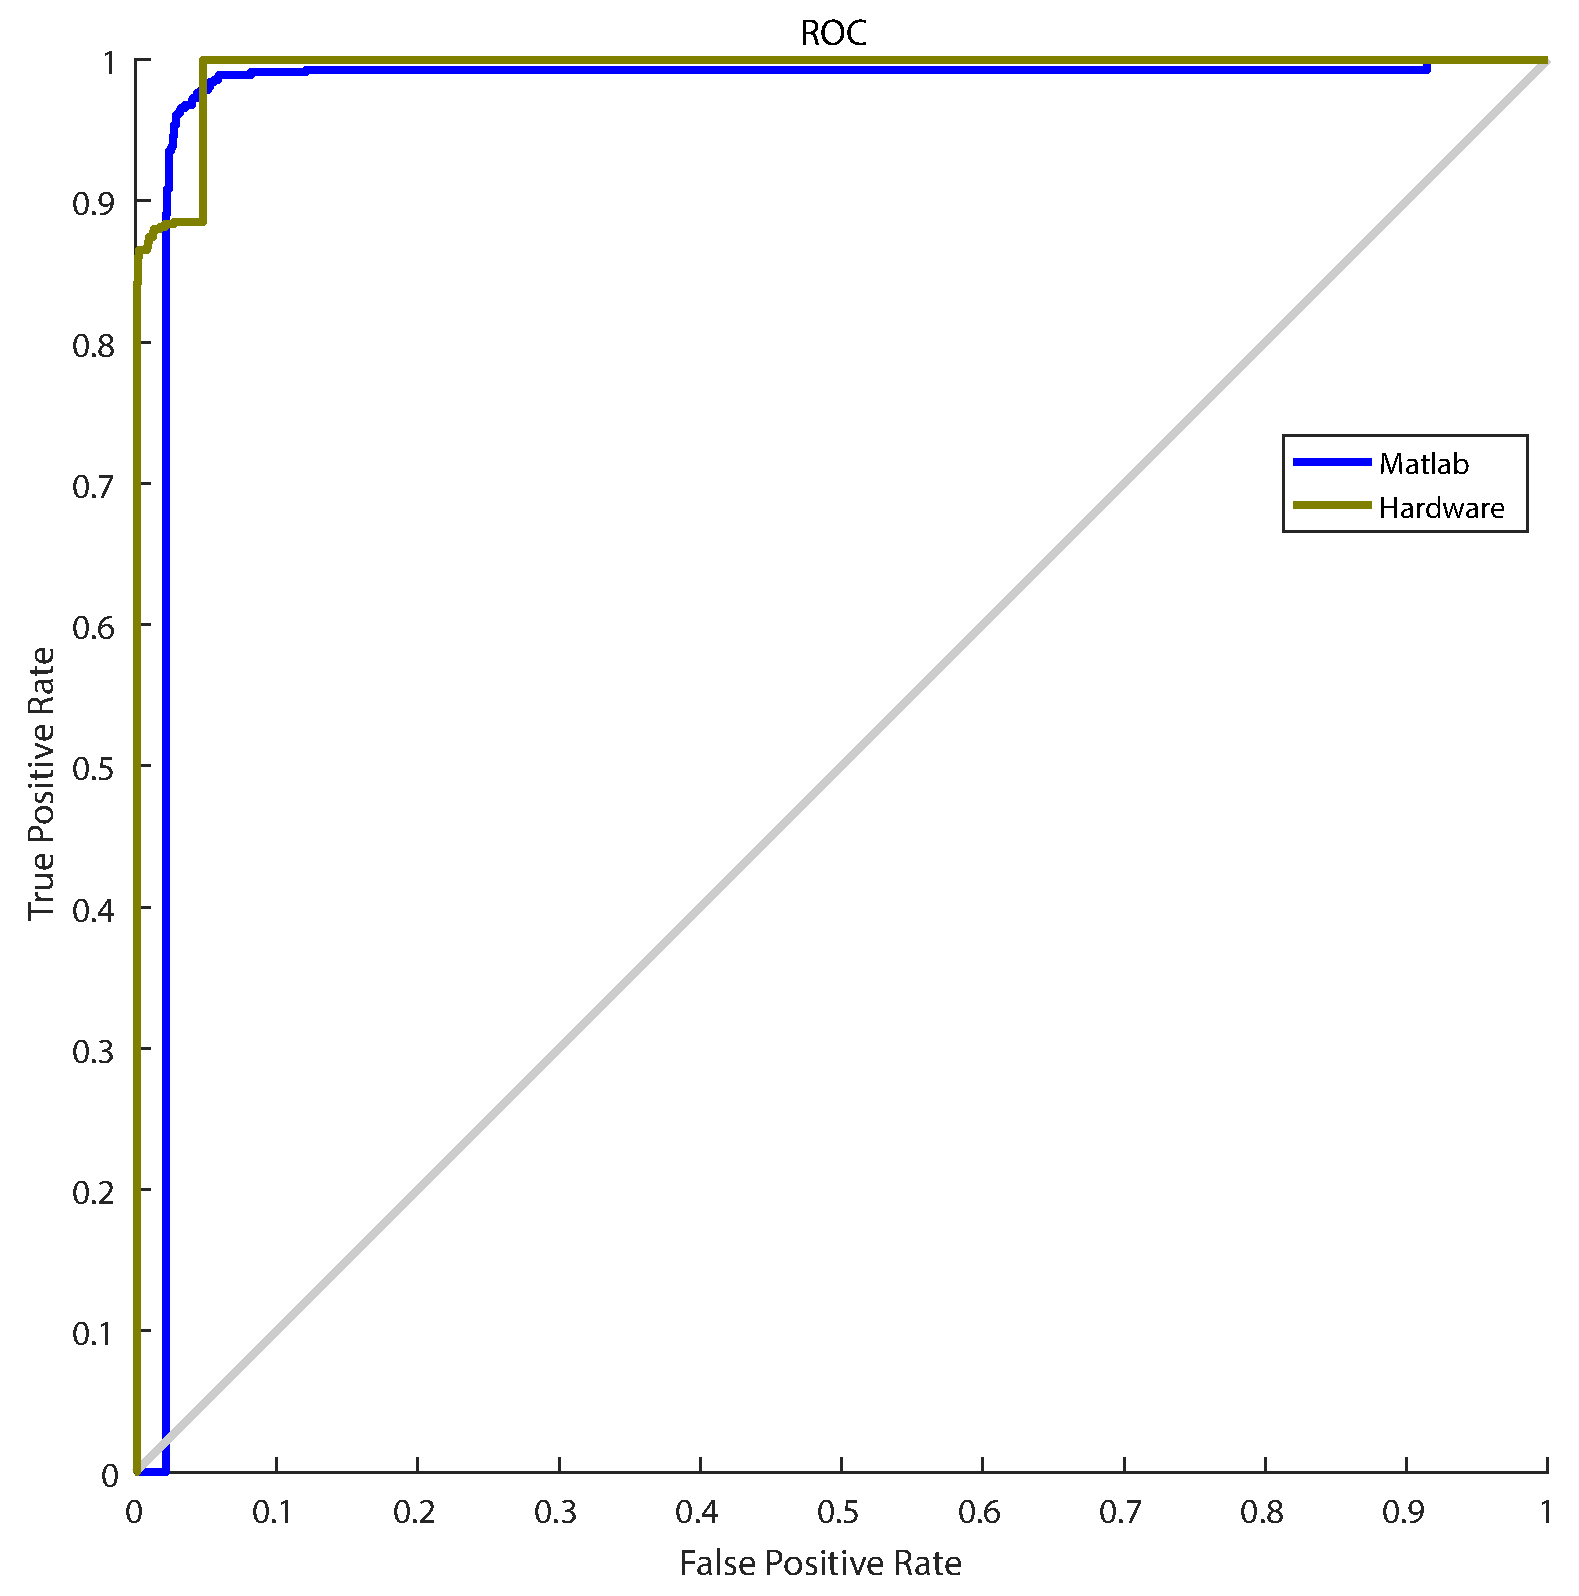
\includegraphics[scale=0.35]{./Figures/ROCANN}
	\caption{Curva ROC de detección}
	\label{fig:ROC}
\end{figure}

 La Figura \ref{fig:ROC} muestra la curva ROC o \textit{Receiver Operating Characteristic} por sus siglas en inglés. Esta gráfica lo que muestra es la calidad del clasificador al discriminar entre un valor de detección positivo y otro negativo basado en el conjunto de datos de entrenamiento. Particularmente, una curva ROC muestra lo siguiente según su forma \citep{ROCCurve}:
 
 \begin{itemize}
     \item Se muestra el balance entre la sensibilidad (eje vertical) y la especificidad (eje horizontal), donde un incremento en la sensibilidad va acompañado de un detrimento de la especificidad.
     \item Entre más cerca la curva esté al eje vertical izquierdo y al eje horizontal superior, más efectivo es el clasificador.
     \item Entre más cerca esté la curva a la diagonal, menos efectivo es el clasificador.
 \end{itemize}
 
A partir de la curva ROC es entonces posible determinar que el modelo se encuentra en capacidad de detectar eficazmente el riesgo de inundación y que el modelo en Matlab presenta un desempeño aceptable para el propósito planteado, cual es el de presentar una plataforma de computación de borde con capacidad de acelerar el procesamiento y análisis de múltiples fuentes de datos. Por ello, no se invirtió más tiempo en sintonizar los parámetros de entrenamiento del modelo, lo que ocasiona que este presente algunas detecciones falsas; esto mayoritariamente se debe a las fluctuaciones generadas por el transitorio entre los estados de inundación y sequía propios del conjunto de datos, generando falsos positivos y/o negativos. Esto es posible corregirlo ajustando los parámetros del entrenamiento a tal punto que las fluctuaciones en la detección sean menos notorias, pero particularmente para este problema las transiciones podrían seguir presentes. Ajustando la salida de la ANN con un circuito de retraso que pueda amortiguar los cambios de estado permitiría filtrar la salida de la ANN de tal forma que no se vea afectada la medición final.

Finalmente, se hace necesario comparar punto a punto la salida de la ANN con el fin de determinar que, efectivamente tanto el modelo en Matlab como su correspondiente implementación en hardware, están entregando una equivalencia para el conjunto de datos entregado. Para ello se eligió calcular el índice de correlación y la correlación cruzada. En el primer caso, el índice de correlación es de $0.9329$, siendo un valor de $1$ una perfecta relación positiva entre dos señales \citep{correlation2,correlation}. La Figura \ref{fig:xcorr} muestra la correlación cruzada entre las señales provenientes del modelo de Matlab y el calculado con el entrenamiento sobre el hardware. Se ve claramente que, según la teoría, la forma triangular sugiere que se trata de una correlación entre dos señales muy similares entre sí, confirmando que el entrenamiento y la detección de ambas redes es equivalente.

\begin{figure}[!ht]
	\centering
		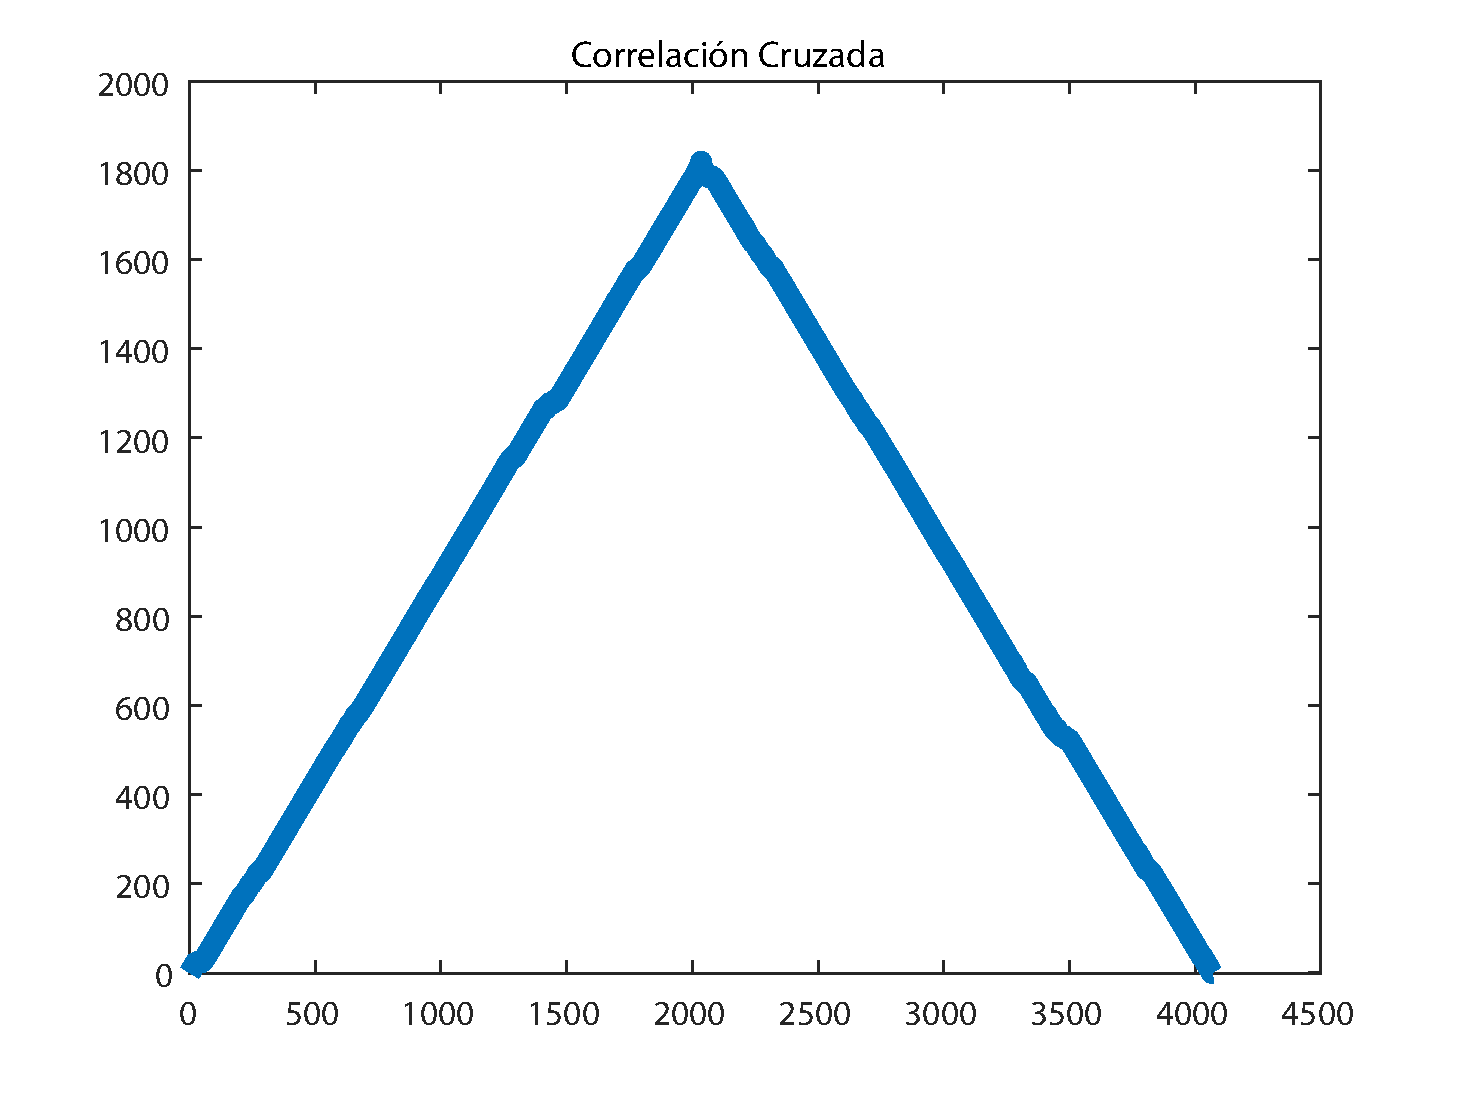
\includegraphics[scale=0.6]{./Figures/xcorrANN}
	\caption{Correlación cruzada entre modelos}
	\label{fig:xcorr}
\end{figure}

%Los resultados de detección para la red neuronal aquí expuestos implican que es posible usar configuraciones de redes neuronales mucho más complejas que en Matlab son muy simples de configurar y que los resultados del entrenamiento puedan ser llevados a la implementación Hardware sin dudas que la variación en la detección cambie drásticamente sin necesidad de implementar complejos algoritmos de entrenamiento usando C/C++ directamente sobre el hardware como aquí se propuso.
